\documentclass[aspectratio=1610]{beamer}
\usetheme{Berlin}
\usepackage{xeCJK}
\setCJKmainfont{SimSun}
\usepackage{multirow}
\usepackage{graphicx}
\usepackage{booktabs} % for better table formatting
\usepackage{geometry} % for adjusting page layout
\usepackage{enumitem} % for customizing lists
\usepackage{hyperref} % for clickable links and references
\usepackage{subcaption}
\usepackage{tikz}
\usetikzlibrary{quantikz}

\title[Mid-term]{基于TDD的量子模型检测中的可达性分析}
\subtitle{硕士中期报告}
\author[Gcc]{高丁超\\ 导师:应圣钢}
\institute[ISCAS]{Institute of Software Chinese Academy of Sciences}
\AtBeginSection{
    \begin{frame}
        \frametitle{Table of Contents}
        \tableofcontents
    \end{frame}
}
\begin{document}
\begin{frame}[plain]
    \titlepage
    \begin{figure}
        \centering
        \begin{subfigure}[c]{0.4\textwidth}
            \centering
            \includegraphics[height= 2cm]{Img/iscas.png}
        \end{subfigure}
        \qquad
        \begin{subfigure}[c]{0.4\textwidth}
            \centering
            \includegraphics[height= 2cm]{Img/ucas.jpg}
        \end{subfigure}
    \end{figure}
    %  Title page
\end{frame}
\section{Requirements for Graduation}
\begin{frame}{Credit Requirements}
    \begin{itemize}
        \item \textbf{Credit Requirement Summary:}
        \begin{itemize}
            \item \textit{Public Compulsory Courses:} 7 credits
            \item \textit{Public Elective Courses:} Minimum 2 credits
            \item \textit{Major Degree Courses:} Minimum 12 credits
            \item \textit{Total Credit Requirement:} Minimum 30 credits
        \end{itemize}
        \item \textbf{Completed Credits:}
        \begin{itemize}
            \item \textit{Public Compulsory Courses:} 7 credits
            \item \textit{Public Elective Courses:} 8 credits
            \item \textit{Major Degree Courses:} 18 credits
            \item \textit{Total Credits Earned:} 35 credits
        \end{itemize}
    \end{itemize}
\end{frame}
\begin{frame}{Research Requirements}
    \begin{itemize}
        \item \textbf{Publication Requirements:}
        \begin{itemize}
            \item Required to be among the top 3 authors on a paper in CCF-A/B category.
        \end{itemize}
        \item \textbf{Completed Submissions:}
        \begin{itemize}
            \item \textit{ICCAD 2023 (CCF-B):}
            \begin{itemize}
                \item Review Outcome: Rejected
                \item Reviewer Scores: 2, 4, 4
            \end{itemize}
            \item \textit{DAC 2024 (CCF-A):}
            \begin{itemize}
                \item Current Status: Under Review
                \item Expected Feedback Date: On or before February 26, 2024
            \end{itemize}
        \end{itemize}
    \end{itemize}
\end{frame}

\section{Backgroud}

\begin{frame}
    \begin{itemize}
        \item \textbf{Title:} 基于TDD的量子模型检测中的可达性分析
        \item \textbf{Summary:}
        \begin{itemize}
            \item \textit{Problem:} How to verify propositions in a quantum system.
            \item \textit{Solution:} Employ Quantum Model Checking.
            \item \textit{Challenge:} Exponential resource requirements with increasing qubits.
            \item \textit{Method:} Utilization of specialized data structures and algorithms.
        \end{itemize}
    \end{itemize}
\end{frame}
\begin{frame}{Quantum Compuating Key Concepts}
    \begin{itemize}[itemsep=18pt]
        \item \textbf{Qubits} 
        \item \textbf{Quantum Gates} 
        \item \textbf{Superposition} 
        \item \textbf{Entanglement}
    \end{itemize}
\end{frame}
\begin{frame}{Quantum Compuating example}
    \begin{figure}[h]
      \centering
      \scalebox{1.1}{
      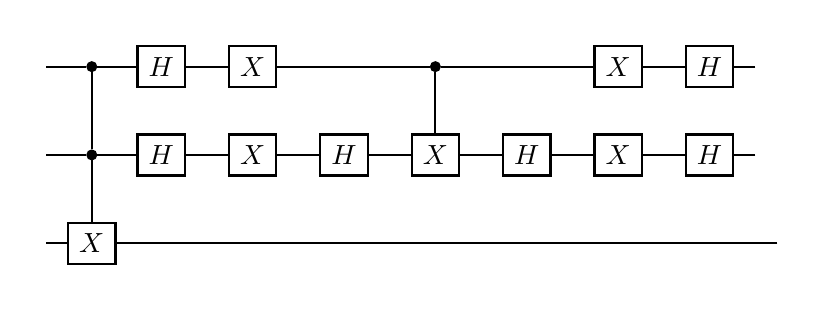
\begin{tikzpicture}
      \node at (0,0) [anchor=north]{
      \begin{quantikz}[column sep=0.28cm,row sep=0.6cm]
      &\ctrl{1}&\gate{H}&\qw&\gate{X}&\qw&\qw&\qw     &\ctrl{1}&\qw&\qw&\qw     &\gate{X}&\qw&\gate{H}&\qw \\
      &\ctrl{1}&\gate{H}&\qw&\gate{X}&\qw&\gate{H}&\qw&\gate{X}&\qw&\gate{H}&\qw&\gate{X}&\qw&\gate{H}&\qw \\
      &\gate{X}&\qw     &\qw     &\qw     &\qw     &\qw     &\qw     &\qw     &\qw&\qw&\qw&\qw&\qw&\qw&\qw&\qw 
      \end{quantikz}};
      \end{tikzpicture}
      }
      \caption{ Quantum circuit of Grover algorithm}
      \end{figure}
\end{frame}

\begin{frame}{Quantum Transition System}
    \begin{itemize}
        \item  \textbf{transition system:} $(S, I, \Sigma, T)$
        \begin{equation}
          where
          \begin{cases}
            x = x_1, \cdots, x_n\\
            y = y_1, \cdots, y_n\\
            \sigma = \sigma_1, \cdots, \sigma_m
          \end{cases}
          \notag
        \end{equation}
        \item \textbf{Quantum transition system:} $(\mathcal{H}, \mathcal{H}_0, Act, \{U_\alpha,\alpha\in Act\})$
    \end{itemize}
\end{frame}
\begin{frame}{Reachability problem}
    \begin{figure}
        \includegraphics[width=.6\textwidth]{Img/eventually.png}
    \end{figure}
    \begin{figure}
        \includegraphics[width=.6\textwidth]{Img/eventuallyalways.png}
    \end{figure}
    \begin{figure}
        \includegraphics[width=.6\textwidth]{Img/alwayseventually.png}
    \end{figure}
  \end{frame}
\begin{frame}{Quantum Logic}
    \begin{itemize}
        \item \textbf{Subset relation \( \subseteq \) in \(S(\mathcal{H})\):} Partial order, implies quantum implication.
        \item \textbf{Orthogonal complement \( \mathcal{X}^\perp \):} Represents negation.
        \item \textbf{Closed under intersection:} \( \bigcap_{i} \mathcal{X}_{i} \in S(\mathcal{H}) \), denotes conjunction.
        \item \textbf{Union of subspaces:} \( \bigvee_i \mathcal{X}_i = \text{span} \left( \bigcup_i \mathcal{X}_i \right) \), interprets disjunction.
    \end{itemize}
\end{frame}
\begin{frame}{Quantum Model Checking example}
    \begin{figure}
      \includegraphics[width=.9\textwidth]{Img/early.png}
      \caption{ the purpose of early research}
    \end{figure}
\end{frame}
\begin{frame}{Quantum Model Checking example}
    \begin{figure}
        \centering
        \begin{subfigure}{0.3\textwidth}
          \includegraphics[width=\textwidth]{Img/rus1.png}
        \end{subfigure}
        \quad
        \begin{subfigure}{0.3\textwidth}
          \includegraphics[width=\textwidth]{Img/rus2.png}
        \end{subfigure}
        \caption{ Circuit Equivalence Checking}
    \end{figure}
\end{frame}
\begin{frame}{Tensor Decision Diagram}
    \begin{figure}
        \begin{subfigure}{0.4\textwidth}
            \includegraphics[height=3.5 cm]{Img/matrix_of_tdd.pdf}
            \label{fig:mat_P}
        \end{subfigure}
        \qquad
        \qquad
        \qquad
        \begin{subfigure}[c]{0.4\textwidth}
            \centering
            \includegraphics[height=6cm]{Img/tdd_ex.pdf}
            \label{fig:tdd_P}
        \end{subfigure}
        \label{fig:P}
    \end{figure}
\end{frame}

\section{Our Soulution}
\begin{frame}{Related work}
    \begin{figure}
      \includegraphics[height=4.5cm]{Img/QMDD.png}
    \end{figure}
  \end{frame}
\begin{frame}{Related work}
    \begin{figure}
        \includegraphics[height=4cm]{Img/tdd-compare.pdf}
        \caption{ time consumption for constructing the functionality of qft circuits}
    \end{figure}
\end{frame}
\begin{frame}{Additional}
    \begin{figure}
        \centering
        \includegraphics[height=4cm]{Img/cir_index_graph.pdf}
        \caption{ addition partition}
    \end{figure}
\end{frame}
\begin{frame}{Contraction}
    \begin{figure}
        \centering
        \includegraphics[height=4cm]{Img/cir_contraction.pdf}
        \caption{ contraction partition}
    \end{figure}
\end{frame}
\begin{frame}{Results}
    \begin{table}[]
        \scalebox{1.1}{
            
        \rule{0pt}{30pt}
        \begin{tabular}{l|ccc}
        benchmark & basic & addition& contraction \\\hline
        Grover 20       & $\sim$5min  & $\sim$4min & $\sim$4sec  \\
        Quantum Fourier Transform 20           & $\sim$20min & $\sim$11min & $<$1sec \\
        Quantum Random walk 20           & $\sim$6min & $\sim$4min & $\sim$15sec\\
        Bernstein-Vazirani 50           & $\sim$4min & $\sim$4min & $\sim$16sec \\
        GHZ 500         & $\sim$3sec & $\sim$1.5sec & $\sim$1.7sec\\
        \end{tabular}
        }
        \caption{Quantum Image computation}
    \end{table}
\end{frame}
\begin{frame}{Local Invertible Map-DD}
    \begin{figure}
        \begin{subfigure}{0.4\textwidth}
            \centering
            \includegraphics[height=5cm]{Img/limdd.pdf}
        \end{subfigure}
        \begin{subfigure}{0.4\textwidth}
            \centering
            \includegraphics[height=5cm]{Img/limdd_reduce.pdf}
        \end{subfigure}
        \caption{ future plan}
    \end{figure}
\end{frame}

\section*{End}
\begin{frame}
    \centering
    \Huge The End
\end{frame}
\end{document}